\subsection{Server}

\subsubsection{\nameref{API}}
\begin{figure}[H]
    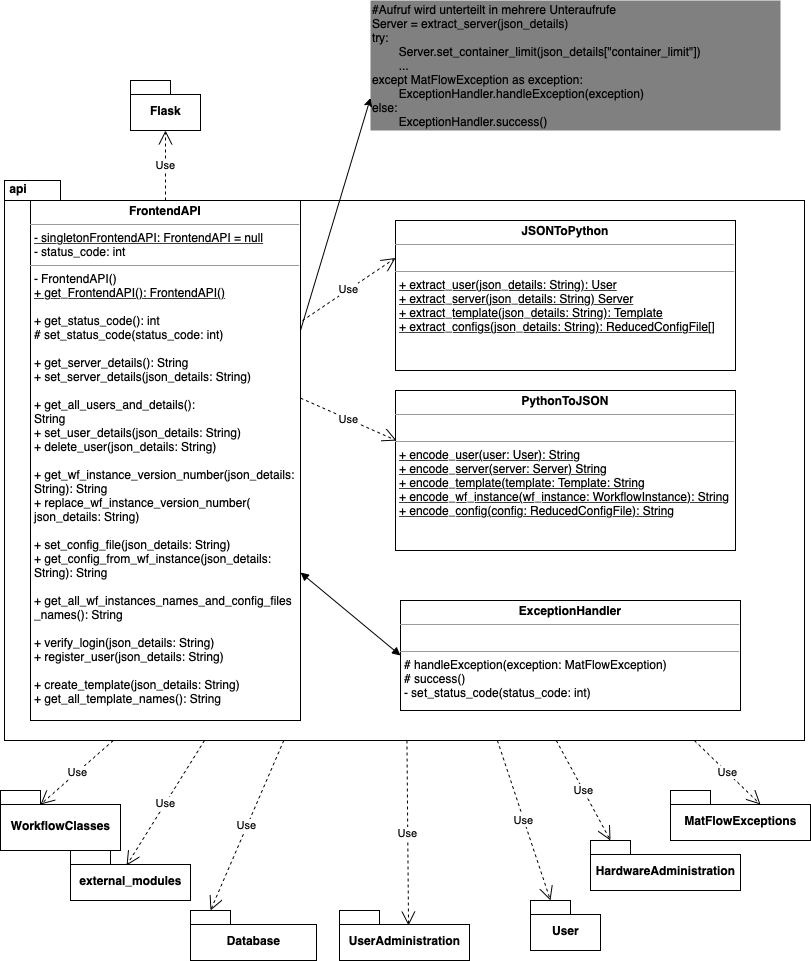
\includegraphics[width=1\textwidth]{res/api.drawio.png}
    \caption{API Package}
\end{figure}
Dieses Package ist zuständig für die Kommunikation zwischen der Client Applikation und der Serverapplikation (siehe Kapitel 
Kommunikation). Anfragen an die Klasse FrontendAPI werden an die dementsprechenden packages weitergeleitet, wo diese konkret 
ausgeführt werden. Diese Klasse fängt alle Exceptions und leitet sie an die Klasse ExceptionHandler weiter.
In der ExceptionHandler Klasse wird dann der Status Code der FrontendAPI Klasse geändert, der für den Client aussagekräftig
darüber ist welcher Fehler geworfen wurde.

\subsubsection{MatFlowExceptions}
\begin{figure}[H]
    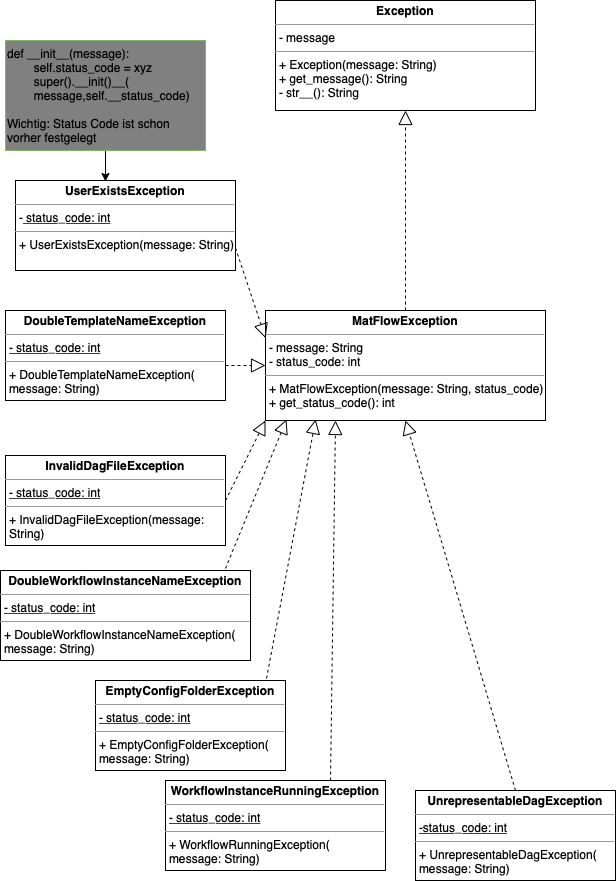
\includegraphics[width=1\textwidth]{res/Klassen/MatFlowExceptions.png}
    \caption{MatFlowExceptions}
\end{figure}
Dieses Package beinhaltet alle MatFlowExceptions. Diese werden geworfen, wenn es einen MatFlow spezifischen Fehler, ausgelöst 
durch den Nutzer, in der Anwendung gibt.


\newpage